\section{第二类:两遍的方式}
对于探测哪些表面是从光源不可见的,和探测哪些表面是从视点不可见的,隐藏表面算法都很容易使用。
但是,为了有用,算法必须生成能被利用的信息,用来在下一遍计算中生成从出射点看到的图片。
这个限制限定了可应用的算法的类别。\\
Sutherland, Sproull 和 Schumaker提出了一种隐藏表面算法,可以分为物体空间算法和图像空间算法\cite{12}。
这种区分是很重要的,因为必须在物体空间里决定阴影的边界,这样生成的信息才能合并进发送到显示算法的数据中。
因为图像空间算法基于显示媒体的有限分辨率,所以用图像空间算法来减轻决定隐藏表面的负担对于这类应用来说是不恰当的。\\
由Sutherland等人描述的算法\cite{12}都严格地在物体空间上操作,都有令人沮丧的增长律(计算复杂度是数据数量的平方)。
此外,当考虑多边形时,它们不是被当作整体,而是被分成了独立对待的面。
为了产生阴影,多边形必须被当作整体,这样它们才能被阴影边界划分开,然后作为更小的多边形返回给数据库,并传递给显示算法。
忽略物体空间算法,剩下了由Newell, Newell和Sancha提出的算法\cite{9}。
这个算法提供了很多有用的技术用来分离多边形和决定重叠部分。
但是最终决定哪个部分的哪个表面是隐藏的,还是通过覆写图像空间来完成的。\\
Sutherland提出了另一种对于此问题更实用的算法\cite{11}。
使用裁剪技术,执行一次二分排序,可以发送多边形和一条线一侧的多边形侧面部分到一条流数据上,而另一侧的侧面部分到另一条流数据上。
当然这种步骤正是决定表面有阴影部分和无阴影部分的划分所需要的。
此外,Sutherland的算法有一个合理的增长速率保证。
因为算法利用对数据的二维二分排序,通过对视场空间的递归划分,可以得到一个$ N\log N $ 的增长律。\\
Sutherland还提出了改进,在子划分的过程中只考虑“轮廓”边。
轮廓边是指分开正面多边形和背面多边形的那些边。
在这些地方,表面曲线会隐藏在自身后面,或者其他表面边缘的边后面。
而这些表面自身没有封闭\cite{1}。
所以,任何区域,只要在单个表面的一组轮廓边的边界内,就可以认为是一个单元,并且假设围起来的表面就是围起来的区域的最前面。\\
Clark提出了一个实现隐藏表面算法的通用模式,用到了对于一种层次化数据描述的递归下降法\cite{7}。
通过将这种方式和Sutherland的轮廓裁剪标注法组合起来,可以保证一个有趣的阴影算法。
如果可以强加一个环境限制:物体一定可以分成线性可分的子物体,和线性可分子物体的组合,那么可以通过以下方式实现一个算法。\\
算法第一步是用和Newell,Newell和Sancha相似的排序技术,来建立一个从正面到背面的待考察表面的优先级顺序。
Clark提出的层次化方法可以叠加到第一顺序的物体或者物体组,然后在这些物体或物体组内再建立一个顺序。
Newell最近建议说,在这里可以应用将物体排序成深度优先顺序的算法\cite{10}。\\
注意到,为了探测阴影,物体的外围可能用来确定一个“印迹”,或者在透视投影下的反窗口。
任何在“印迹”里的东西,并且离光源很远的话,在阴影里都会清除掉。
所以,我们可以交替使用每个顶点子物体的外围来增强一组“印迹”,这样来进行算法。
远离光源,被“印迹”隐藏的表面可以标记为有阴影的。
其他表面将它们外围无阴影的部分添加到“印迹”集合中,然后被裁剪成有阴影和无阴影的部分。\\
通过一个可以提供相邻多边形之间链接的数据结构,找到多边形物体的外围是很容易的。
这种数据结构在\cite{6}\cite{8}中有详细表述。
因为外围是从轮廓边里单独形成的,而且一个顶点表面的所有轮廓边都一定在外围内,所以决定外围的过程包含了找到轮廓边的闭环。\\
轮廓边的串可以很直观地形成。
首先,相对于光源的视角,所有多边形必须被标记为正面,或者背面。
然后,必须检查每个正面多边形的邻居多边形。当找到背面相邻多边形时,它的关联边必须被标记为外围边。
最后,通过使用相邻的正面多边形来搜索连接到一个已知外围顶点的额外外围边,外围边可以连接起来。
对于一个顶点物体,单个的边串可以形成它的外围(图\ref{fig:fig2})。\\
\begin{figure}[h]
\centering
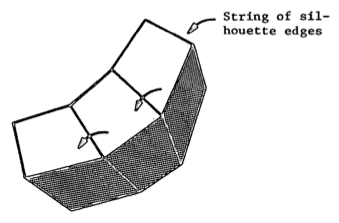
\includegraphics[width=0.9\linewidth]{fig2}
\caption[fig2]{通过搜索相邻正面多边形的轮廓边,可以形成外围边的串。}
\label{fig:fig2}
\end{figure}
通过使用Clark提出的模式,有些物体的外围的计算可以避免。
利用数据的层次性划分(组,物体,子物体),用“界限盒”的测试方法,可以用来决定哪组会从光源视角重叠。
界限盒是用物体顶点的宽高范围决定的(图\ref{fig:fig3})。
\begin{figure}[h]
\centering
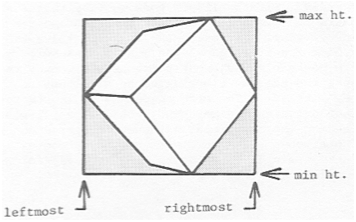
\includegraphics[width=0.9\linewidth]{fig3}
\caption[fig3]{"界限盒“}
\label{fig:fig3}
\end{figure}
任何时候,发现一个物体的界限盒完全在一个更高优先级物体的外围内时,前者物体就在阴影里了。
类似地,如果一个顶点物体(由单个子物体组成)的界限盒没能重叠任何其他物体,那么这个物体显然就不在任何阴影中。
在这种情况下,就没理由要计算外围了。\\
可以用数据的层次结构驱动阴影算法。
所以物体组可以按优先级顺序处理,最近者优先。
在每组物体中,物体会按优先级顺序处理。
在每个物体内,子物体也会按优先级顺序处理。
重叠测试会先确定组间是否有交叉。
如果有,那么界限盒就要传递到下一级更低的层级中。
然后重叠测试会应用到组内的物体间,最终到每个物体的子物体间。
如果一个子物体的界限盒没有和任何层间传递下来的界限盒重叠,那么就可以忽略它了。
否则的话,就要计算它的外围。\\
按照要求计算出高优先级的子物体的外围后,内部物体的阴影边界就可以计算了。
这个计算可以通过在高优先级子物体的外围内裁剪出低优先级子物体的多边形来完成。
如果任何低优先级的子物体是完全阴影覆盖的,那么它就可以标记为完全阴影的,并在之后的重叠测试中忽略掉。
部分阴影覆盖的子物体会被裁剪为有阴影部分和无阴影部分。
然后仅基于无阴影的部分,可以计算出部分的外围。
完全没有被阴影覆盖的子物体仅仅算出了它们的外围而已。\\
当算法按着物体序列的优先级顺序进行运算时,一个顶点印迹的最小集合会构建出来,每个印迹都有与之关联的界限盒。
当处理低优先级的物体时,它们会被更高优先级的印迹裁剪,然后余下的多边形会被用来计算部分外围,结果会加到印迹的集合中。
提前准备将一组印迹吸收进单个印迹中是有用的,以防低优先级的子物体足够大,以至于可以提供一个包裹的外围。
但是,对于这种情况的检查的开销被证实会大于它所带来的益处。\\
当有几组物体重叠时,在所有低优先级组处理完后,很有可能会构建出一个极大的印迹集合。
为了避免过度增长的计算量,印迹的集合和未处理数据应该分区,这样部分分开的区域可以单独处理。
利用界限盒提供的信息,分区会变得简单。
甚至随着印迹集合的增长,重复多分区几次是有利的。
另外,基于低优先级物体的界限盒的分区方式可以将不再需要的印迹丢弃。\\
当然这种方法严重依赖于一个良性条件的环境(顶点子物体)。
并不清楚
(1)该算法是否易于扩展到一般情况 和
(2)数据生成和物体建模技术是否总是可以交付出这样良性条件的数据。\\
一般来讲,上面描述的测试序列会随着包含的物体的数量按平方的复杂度增加开销。
但是,将数据划分成一个层次结构,在印迹数变大时使用分区方式,都会减少必要的测试的数量。
还要再一次指出的是,如果光源在或者靠近出射点的视场时,为了确定阴影,就需要将空间分区,这样透视投影才能派上用场。
这种方法严重依赖于确定正面多边形和背面多边形的难易程度,还依赖于重叠测试。
这两者在一次透视变换后都会变得很容易。\\
一旦阴影多边形确定下来了,任何隐藏表面算法都可以用来从增强的数据中生成出射点图像。
所以,两遍方式的优势就在于,确定阴影的过程和之后图片生成的过程完全独立。
这样阴影处理和图片生成就可以以流水线的形式并行处理了。
注意到,给定两个处理器,如果阴影探测算法和显示算法是分开且并行运行的,那么将阴影检测算法变得比显示算法更高效是毫无意义的。
而且,给定一个静态的环境和固定的光源,对许多出射点位置来讲,阴影只需要计算一次。
在这种情况下,阴影算法的效率变得更无关紧要了。